Все современные дифференциальные алгоритмы слежения за особенностями опираются на работу 1981 году Лукаса и Канаде \cite{Lucas1981}. В 1991 году математическая формулировка этого алгоритма была изменена, и стала основой для всех последующих обобщений с учётом аффинных искажений окрестности и освещённости. Путём замены соответствующих переменных на константы любой из них превращается в обычный алгоритм Лукаса−Канаде \cite{lk_jou}.
\subsection{Описание дифференциального алгоритма определения оптического потока Лукаса−Канаде}

В основе всех дальнейших рассуждений лежит одно очень важное и не очень справедливое предположение: Предположим, что значения пикселей переходят из одного кадра в следующий без изменений. Таким образом, мы делаем допущение, что пиксели, относящиеся к одному и тому же объекту, могут сместиться в какую либо сторону, но их значение останется неизменным. Конечно же это предположение имеет мало общего с реальностью, потому что от кадра к кадру могут меняться глобальные условия освещения и освещённость самого движущегося объекта. Масса проблем связана с этим допущением, но, как ни странно, вопреки всему оно достаточно хорошо работает на практике. На математическом языке это допущение можно записать так:
\numberwithin{equation}{section}
\label{eq:f_0}
\begin{equation}
I(x,y,t)=I(x+u_x,y+u_y,t+1)
\end{equation}

где $I$ — это функция яркости пикселей от положения на кадре и времени. Другими словами $x$ и $y$ — это координаты пикселя в плоскости кадра, и — это смещение, а $t$ — это номер кадра в последовательности. Условимся, что между двумя соседними кадрами проходит единичный отрезок времени.
\subsubsection{Одномерный случай алгоритма}

\begin{figure}[ht]
\center{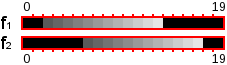
\includegraphics[width=0.4\linewidth]{math_1}}
\caption{Одномерный сдвиг яркостей}
\label{pic:math_1}
\end{figure}

Для начала рассмотрим одномерный случай. Рассмотрим представленные на рисунке \ref{pic:math_1} два одномерных кадра размером 1х20 пикселей. На  рисунке \ref{pic:math_1} кадр $f_2$ смещено вправо на 4 пикселя. Именно это смещение необходимо найти. Для этого представим эти же кадры в виде функций (рисунок \ref{pic:math_2}). На входе позиция пикселя, на выходе — его интенсивность. В таком представление искомое смещение ($d$) видно еще более наглядно. В соответствии с нашим предположением,$f_2$ это просто смещённая $f_1$, то есть можно сказать, что:

\numberwithin{equation}{section}
\label{eq:f_2}
\begin{equation}
f_2(x)=f_1(x-d)
\end{equation}

\begin{figure}[ht]
\center{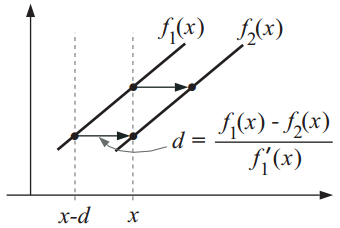
\includegraphics[width=0.4\linewidth]{math_2}}
\caption{Функция зависимости интенсивности от позиции пикселя}
\label{pic:math_2}
\end{figure}

Обратите внимание, что $f_1$ и $f_2$ при желании можно записать и в общем виде: $f_1(x)=I(x,y,t)$ $f_2(x)=I(x,y,t)$ ; где $y$ и $t$ зафиксированы и равны нулю.

Для каждой координаты нам известны значения и в этой точке, кроме того мы можем вычислить их производные. Свяжем известные значения со смещением $d$. Для этого запишем разложение в ряд Тейлора для $f_1(x-d)$:
$$f_1(x-d)=f_1(x)-df^{'}_1(x)+O(d^2f^{''}_1)$$

Сделаем второе важное предположение: Предположим, что достаточно хорошо аппроксимируется первой производной. Сделав это предположение, отбросим всё что после первой производной:
$$f_1(x-d)=f_1(x)-df_1^{'}(x)$$

Насколько это корректно? В общем-то не очень, тут мы теряем в точности, если только наша функция/изображение не строго линейна, как в нашем искусственном примере. Зато это существенно упрощает метод, а для достижения требуемой точности можно сделать последовательное приближение, которе мы рассмотрим позже.

Мы почти у цели. Смещение $d$ — это наша искомая величина. Исходя из \ref{eq:f_2}, сделаем замену:$f_2(x)=f_1(x)-df_1^{'}(x)$
откуда выведем $d = \dfrac{f_1(x)-f_2}{f_1^{'}(x)}$
\subsubsection{Двумерный случай алгоритма}

Теперь перейдём от одномерного случая к двумерному. Запишем разложение в ряд Тейлора для \ref{eq:f_0} и сразу отбросим все старшие производные. Вместо первой производной появляется градиент:
$$I(x+u_x,y+u_y,t+1)=I(x,y,t)+\overrightarrow{u} \nabla I(x,y,t)$$
где $\overrightarrow{u} = \begin{bmatrix}
u_x\\
u_y
\end{bmatrix} $ — вектор смещения.
В соответствии со сделанным допущением \ref{eq:f_0}. Перепишем:
$$I(x,y,t)-I(x_x,y_y,t+1) + \overrightarrow{u} \nabla I(x,y,t) = 0$$
Поскольку между двумя кадрами проходит единичный интервал времени, то можно сказать, что $I(x,y,t)-I(x,y,t+1)$ есть не что иное, как производная по времени.
Заменим:
$$\frac{\partial I(x,y,t)}{\partial t} + \overrightarrow{u} \nabla I(x,y,t) = 0$$
Перепишем ещё раз, раскрыв градиент:
$$\frac{\partial I(x,y,t)}{\partial t} + u_x\frac{\partial I(x,y,t)}{\partial x} + u_y\frac{\partial I(x,y,t)}{\partial y} = 0$$

Мы получили уравнение, которое говорит нам о том, что сумма частных производных должны быть равна нулю. Проблема только в том, что уравнение у нас одно, а неизвестных в нем два: $u_x$ и $u_y$. На этом моменте начинается полет фантазии и разнообразие подходов.

Сделаем третье предположение: Предположим, что смещение пикселей между двумя кадрами невелико. Рассмотрим пиксель $p$, тогда, по алгоритму Лукаса — Канаде, оптический поток должен быть одинаков для всех пикселей, находящихся в окне с центром в $p$. А именно, вектор оптического потока $u_x$ и $u_y$ в точке $p$ должен быть решением системы уравнений. Очевидно, что в общем случае система не имеет решения, поэтому будем искать такие $u_x$ и $u_y$, которые минимизируют ошибку:
$$
\begin{cases}
I_x(q_1) V_x + I_y (q_1) V_y = -I_t(q_1)\\
I_x(q_2) V_x + I_y (q_2) V_y = -I_t(q_2)\\
...\\
I_x(q_n) V_x + I_y (q_n) V_y = -I_t(q_n)\\
\end{cases}
$$
где $q_1,q_2,\dots,q_n$ — пиксели внутри окна
$I_x(q_i),I_y(q_i),I_t(q_i)$ — частные производные изображения $I$ по координатам $x$, $y$ и времени $t$, вычисленные в точке $q_i$.
Это уравнение может быть записано в матричной форме:
$$A v = b$$

$$A = \begin{bmatrix}
I_x(q_1) && I_y(q_1) \\
I_x(q_2) && I_y(q_2) \\
\vdots  && \vdots  \\
I_x(q_n) && I_y(q_n)
\end{bmatrix},
\quad\quad
v =
\begin{bmatrix}
V_x\\
V_y
\end{bmatrix},
\quad\quad
b =
\begin{bmatrix}
-I_t(q_1)\\
-I_t(q_2)\\
\vdots \\
-I_t(q_n)
\end{bmatrix} $$
Полученную переопределенную систему решаем с помощью метода наименьших квадратов. Таким образом, получается система уравнений $2 \cdot 2$:
$$A^T A v=A^T b$$
откуда
$$\mathrm{v}=(A^T A)^{-1}A^T b$$
где $A^T$ — транспонированная матрица $A$. Получаем:
$$\begin{bmatrix} V_x\\[10pt] V_y \end{bmatrix} = \begin{bmatrix} \sum_i I_x(q_i)^2 & \sum_i I_x(q_i)I_y(q_i) \\[10pt] \sum_i I_x(q_i)I_y(q_i) & \sum_i I_y(q_i)^2 \end{bmatrix}^{-1} \begin{bmatrix} -\sum_i I_x(q_i)I_t(q_i) \\[10pt] -\sum_i I_y(q_i)I_t(q_i) \end{bmatrix}$$

Вот собственно и все. Мы знаем приблизительное смещение пикселей между двумя соседними кадрами.

Поскольку в нахождении смещения каждого пикселя участвуют также соседние с ним пиксели, при реализации данного метода целесообразно предварительно посчитать производные кадра по горизонтали и вертикали.
\subsubsection{Недостатки метода}

Описанный выше метод основан на трёх значительных допущениях, которые с одной стороны дают нам принципиальную возможность определить оптический поток, но с другой стороны вносят погрешность. Хорошая новость для перфекционистов состоит в том, что одно допущение нужно нам только для упрощения метода, и с его последствиями мы можем бороться. Мы предполагали, что для аппроксимации смещения нам будет достаточно первой производной. В общем случае это конечно же не так (рисунок \ref{pic:math_3}). Для достижение требуемой точности смещение для каждой пары кадров (назовём их $F_i$ и $F_{i+1}$) можно вычислять итеративно. В литературе это называется искажением (warping). На практике это означает, что, вычислив смещения на первой итерации, мы перемещаем каждый пиксель кадра в противоположную сторону так, чтобы это смещение компенсировать. На следующей итерации вместо исходного кадра $F_{i+1}$ мы будем использовать его искажённый вариант $F_{i+1}^1$. И так далее, пока на очередной итерации все полученные смещения не окажутся меньше заданного порогового значения. Итоговое смещение для каждого конкретного пикселя мы получаем как сумму его смещений на всех итерациях.

\begin{figure}[ht]
\center{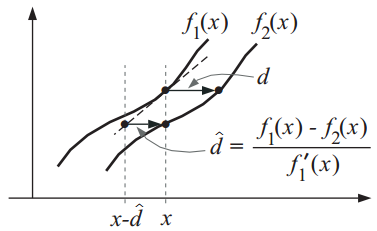
\includegraphics[width=0.4\linewidth]{math_3}}
\caption{Функция зависимости интенсивности от позиции пикселя}
\label{pic:math_3}
\end{figure}

По своей природе данный метод является локальным, то есть при определении смещения конкретного пикселя принимается во внимание только область вокруг этого пикселя — локальная окрестность. Как следствие, невозможно определить смещения внутри достаточно больших (больше размера локальной окрестности) равномерно окрашенных участков кадра. К счастью на реальных кадрах такие участки встречаются не часто, но эта особенность все же вносит дополнительное отклонение от истинного смещения.

\begin{figure}[ht]
\center{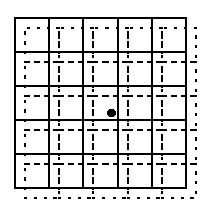
\includegraphics[width=0.4\linewidth]{grid_}}
\caption{Окрестность с субпиксельной точностью}
\label{pic:grid}
\end{figure}

Если интервал времени между кадрами принять за 1, получается следующий алгоритм:
$$\begin{cases} d_k = 0 &\mbox{if } k = 0 \\
d_{k+1}=d_k + C^{-1} \sum_W \left[ (I(x,t) - I(x+d_k,t + 1)) \nabla I (x,t) \right] & \mbox{if } k > 0 \end{cases}
$$
Таким образом, этот алгоритм слежения фактически является поиском точки, в которой достигается минимум некоторой функции, методом градиентного спуска. Во время каждой итерации мы сдвигаемся вдоль направления градиента изображения в текущей точке.
\subsection{Учёт аффинных преобразований}

Учёт аффинных искажений хорошо описан в работе Ши Томаси канаде в 1994 году \cite{shi_tom_lyk}. Движение пикселей окна описывается в виде $Ax + d$, где $A$ - матрица $(2 \cdot 2)$, $а d$ - смещение $(2 \cdot 1)$.

Задача слежения за особенностью сводится к проблеме проблема определения параметров движения и искажения окна особенности, при которой минимизируется разность:
$$r=\iint_W [J(\Delta x+d)-I(x)]^2$$
где $W$ - окно особенности, а $w$ - весовая функция (может использовать, а может и быть равна 1 во всем окне), $J(x)$ и $I(x)$ - два изображения.

Выражение дифференцируется относительно параметров движения, и производная приравнивается к 0. Затем система линеаризуется с помощью разложения функции изображения в ряд Тейлора:
$$J(\Delta x+d)= J(x)+g^T(u)$$

Это даст нам линейную $6 \cdot 6$ систему:
$$Tz=a$$
, где в векторе $z$ объединены все искомые параметры:

$$z^T=\begin{bmatrix}
 d_{xx} & d_{yx} & d_{xy} & d_{yy} & d_x & d_y
\end{bmatrix}$$
Вектор ошибки a записывается в виде:
$$a=\iint_W [I(x)-J(x)]\begin{bmatrix}
xg_x\\
xg_y\\
yg_x\\
yg_y\\
g_x\\
g_y
\end{bmatrix}\omega dx$$
А матрицу размерности $6 \cdot 6$ $T$ можно представить следующим образом:
$$T=\iint_W [I(x)-J(x)]\begin{bmatrix}
U & V\\
V^T & Z
\end{bmatrix}\omega dx$$

$$U=\begin{bmatrix}
x^3 g^3_x & x^3 g_x g_y & x y g^3_x & x y g_x g_y \\
x^3g_xg_y & x^3g^3_y & xyg_xg_y & xyg^3_x \\
xyg^3_x & xyg_xg_y & y^3g^3_x & y^3g_xg_y \\
xyg_xg_y & xyg^3_y & y^3g_xg_y & y^3g^3_y
\end{bmatrix}$$

$$V^T=\begin{bmatrix}
xg^3_x & xg_xg_y & yg^3_x & yg_xg_y \\
xg_xg_y & xg^3_y & yg_xg_y & yg^3_y
\end{bmatrix}$$

$$Z=\begin{bmatrix}
g^3_x & g_xg_y \\
g_xg_y & g^3_y
\end{bmatrix}$$

Полученная система решается также итеративно по методу Ньютона-Рафсона.

Если движение считается не аффинным, а просто смещением, то первые четыре элемента искомого вектора $z$ обращаются в 0, и значимыми остаются только последние два. Алгоритм превращается в алгоритм Tomasi-Kanade.
\subsection{Пирамидальная версия алгоритма}

Пирамидальная версия или иерархический метод. В данном алгоритме важным является нахождение хорошего начального приближения для вектора скорости. Для этого обычно применяют пирамидальную версию алгоритма. Ее идея заключается в том, что наряду с исходной парой изображений ( f; g ) рассматривают эти же изображения сжатые в два раза ( f 2 ; g 2 ) , в четыре ( f 4 ; g 4 ) и  т.д.  ( пирамида ).  Вектора  скорости находят  сначала  на  самом  верхнем  уровне  пирамиды и затем спускаются вниз этаж за этажом. На самом верхнем уровне в качестве начального приближения берут нулевой вектор. На нижних уровнях за начальное приближение берут удвоенную скорость, полученную на предыдущем шаге. Все это вместе взятое обеспечивает хорошее сочетание скорости, точности и устойчивости алгоритма  нахождения  межкадрового  движения  в  виде сдвигов \cite{Bouguet2000}.

Каждое изображение последовательности, за исключением первого, получается как свёртка предыдущего изображения со следующим фильтром:
(рис. \ref{pic:pyramid}).
Пирамидальный алгоритм Лукаса - Канаде для поиска потока в точке $(x_0,y_0)$.
\begin{enumerate}
\item По каждому из двух данных изображениям строится пирамида изображений
\item Для $i$ – го изображения пирамиды по первому и второму изображениям применяется классический KLT метод, с вектором начального приближения $2 \cdot d_{i+1}$, где $d_{i+1}$ – вектор потока, полученный на предыдущем уровне пирамиды.
\end{enumerate}
Для самого первого уровня этот вектор принимается равным (0,0).

\begin{figure}[ht]
\center{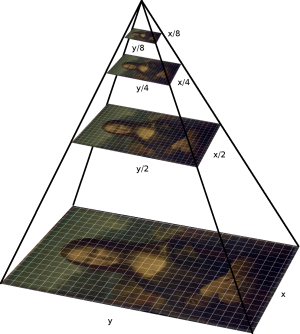
\includegraphics[width=0.6\linewidth]{pyramid}}
\caption{Пример пирамиды Гаусса}
\label{pic:pyramid}
\end{figure}

\subsection{Оценка деформации}

Компоненты рассчитываются путем численного дифференцирования полученного поля смещений. Выражения для продольной $\varepsilon_{xx}$, поперечной $\varepsilon_{yy}$, сдвиговой $\varepsilon_{xy}$ и поворотной $\omega_z$ компонент тензора дисторсии:

$$\varepsilon_{xx}= \frac{\mathrm{d} U_x}{\mathrm{d} x},\varepsilon_{yy}= \frac{\mathrm{d} U_y}{\mathrm{d} y},\varepsilon_{xy}=\frac{1}{2}(\frac{\mathrm{d} U_x}{\mathrm{d} y} + \frac{\mathrm{d} U_y}{\mathrm{d} x}),\omega_z=\frac{1}{2}(\frac{\mathrm{d} U_y}{\mathrm{d} x} - \frac{\mathrm{d} U_x}{\mathrm{d} y})$$

Также выражение для интенсивности деформации сдвига $\gamma_i$

$$\gamma_i = \sqrt\frac{2}{3}\sqrt{(\varepsilon_{xx}-\varepsilon_{xx})^2+\varepsilon_{yy}^2+\varepsilon_{xx}^2 + \frac{3}{2}\varepsilon_{xy}^2}$$